% figures/tikz/graph.tex
% Einfacher ungerichteter Graph mit 4 Knoten
\documentclass[tikz, border=6pt]{standalone}
\usepackage{tikz}
\usetikzlibrary{positioning}

\begin{document}
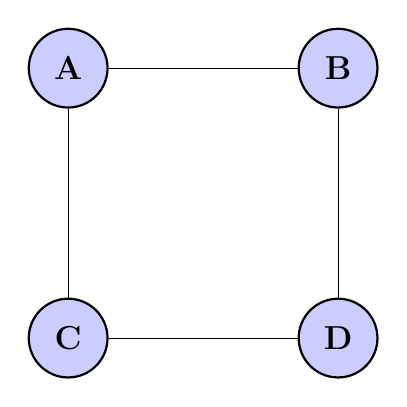
\begin{tikzpicture}[
  every node/.style = {
    circle, draw, thick,
    minimum size = 1cm,
    font = \bfseries\large
  },
  every edge/.style = {draw, thick},
  node distance = 2.4cm
]
  % Knoten
  \node[fill=blue!20]  (A) {A};
  \node[fill=blue!20]  (B) [right=of A] {B};
  \node[fill=blue!20]  (C) [below=of A] {C};
  \node[fill=blue!20]  (D) [right=of C] {D};

  % Kanten
  \draw (A) -- (B);
  \draw (A) -- (C);
  \draw (B) -- (D);
  \draw (C) -- (D);
\end{tikzpicture}
\end{document}
